\documentclass[tikz]{standalone}
\usepackage{pgfplots}

\pgfplotsset{compat=newest}
\pgfplotsset{
    yticklabel style={
        /pgf/number format/fixed,
        /pgf/number format/precision=2
    },
    scaled y ticks=false
}

\begin{document}
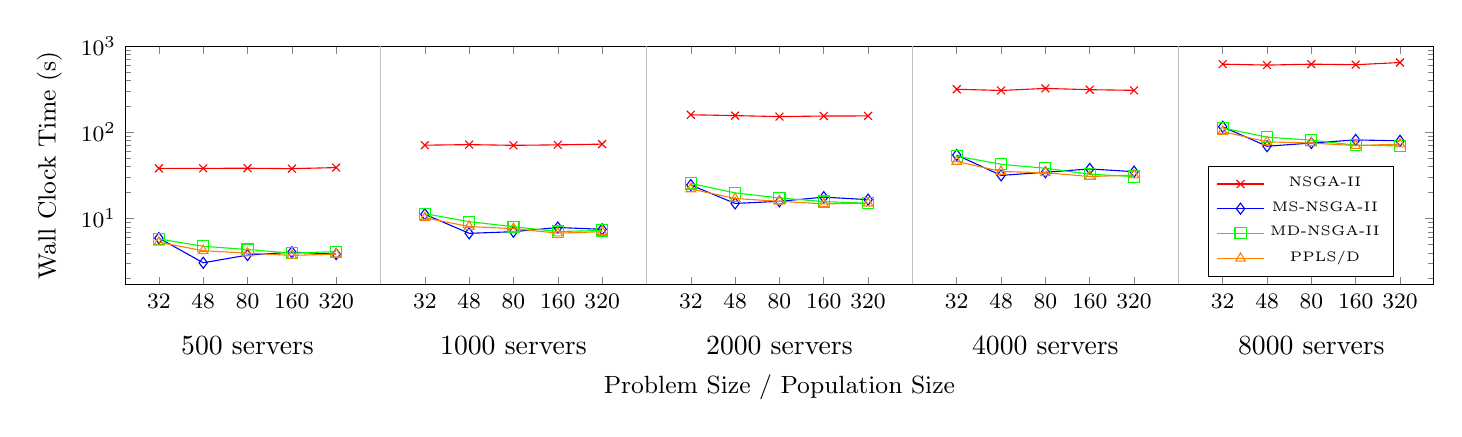
\begin{tikzpicture}

    \begin{axis}[
        footnotesize,
        max space between ticks=20pt,
        width=1.5\textwidth,
        height=0.38\textwidth,
        ymax = 1000,
        try min ticks=5,
        xtick=data,
        xticklabels={32, 48, 80, 160, 320, 32, 48, 80, 160, 320, 32, 48, 80, 160, 320, 32, 48, 80, 160, 320, 32, 48, 80, 160, 320},
        extra x ticks={5,11,17,23},
        extra x tick labels={},
        extra x tick style={
            grid=major,
            major tick length=0pt,
        },
        xlabel={Problem Size / Population Size},
        ylabel={Wall Clock Time (s)},
        xlabel style={
            yshift=-4ex,
        },
        enlarge x limits={abs=0.75},
        legend pos=south east,
        legend entries={
            {NSGA-II},
            {MS-NSGA-II},
            {MD-NSGA-II},
            {PPLS/D},
        },
        clip mode=individual,
        ymode=log,
        legend style={font=\tiny}
    ]

    \addplot[
        mark=x,
        color=red,
    ] table[
        x expr=\coordindex,
        y=TM
    ]{
        PS TM
        32 38.2
        48 38.2
        80 38.3333
        160 37.9
        320 39
        {} {}
        
        32 70.9667
        48 72.0333
        80 70.7
        160 71.5667
        320 73
        {} {}
        
        32 159.9333
        48 156.3333
        80 152.3
        160 154.6
        320 155.1
        {} {}
        
        32 315.9667
        48 306.1
        80 323.3
        160 312.4333
        320 307.1
        {} {}
        
        32 617.9667
        48 603.0333
        80 617.9333
        160 609.2
        320 645.8667
        {} {}              
    };

    \addplot[
        mark=diamond,
        color=blue
    ] table[
        x expr=\coordindex,
        y=TM
    ]{
        PS TM
        32 5.9333
        48 3.0667
        80 3.7667
        160 4.0667
        320 3.8667
        {} {}
        
        32 11.2
        48 6.7333
        80 7.0333
        160 7.8667
        320 7.5
        {} {}
        
        32 24.4333
        48 14.9667
        80 15.8333
        160 17.7
        320 16.5667
        {} {}
        
        32 54.5
        48 31.6667
        80 34.4
        160 37.6333
        320 34.9667
        {} {}
        
        32 115.8667
        48 69
        80 75.1333
        160 81.7
        320 79.7
        {} {}        
    };

    \addplot[
        mark=square,
        color=green
    ] table[
        x expr=\coordindex,
        y=TM
    ]{
        PS TM
        32 5.8
        48 4.7667
        80 4.3667
        160 3.9667
        320 4.1333
        {} {}
        
        32 11.4
        48 9.2
        80 8.0333
        160 7.0667
        320 7.2667
        {} {}
        
        32 25.5333
        48 19.8333
        80 17.3333
        160 15.7333
        320 15.0667
        {} {}
        
        32 52.9667
        48 42.6333
        80 38.3
        160 32.6667
        320 30.7
        {} {}
        
        32 112.3333
        48 88
        80 81.2
        160 70.9333
        320 69.5667
        {} {}               
    };

    \addplot[
        mark=triangle,
        color=orange
    ] table[
        x expr=\coordindex,
        y=TM
    ]{
        PS TM
        32 5.3
        48 4.2333
        80 3.9667
        160 3.7333
        320 3.8667
        {} {}
        
        32 10.2
        48 8.0667
        80 7.6333
        160 6.7667
        320 7.0333
        {} {}
        
        32 22.0333
        48 17.0667
        80 15.8333
        160 14.8
        320 15.0333
        {} {}
        
        32 45.9
        48 35.1667
        80 33.9667
        160 30.7333
        320 31.8667
        {} {}
        
        32 102.0333
        48 77.6333
        80 75.1
        160 70.2333
        320 73.0333
        {} {}                    
    };

    \begin{scope}[
        every label/.append style={
            label distance=2ex,
        },
    ]
        \node [label=below:500 servers, yshift=2.9ex]
            at (axis cs:2,\pgfkeysvalueof{/pgfplots/ymin}) {};
        \node [label=below:1000 servers, yshift=2.9ex]
            at (axis cs:8,\pgfkeysvalueof{/pgfplots/ymin}) {};
        \node [label=below:2000 servers, yshift=2.9ex]
            at (axis cs:14,\pgfkeysvalueof{/pgfplots/ymin}) {};
        \node [label=below:4000 servers, yshift=2.9ex]
            at (axis cs:20,\pgfkeysvalueof{/pgfplots/ymin}) {};
        \node [label=below:8000 servers, yshift=2.9ex]
            at (axis cs:26,\pgfkeysvalueof{/pgfplots/ymin}) {};
    \end{scope}
    \end{axis}
\end{tikzpicture}
\end{document}